\sectionframe{Label Distribution Smoothing (LDS)}
\begin{frame}{Imbalanced Categorical vs. Continuous Label Space (1/3)}
	\begin{figure}[h]
		\begin{subfigure}{0.48\textwidth}
			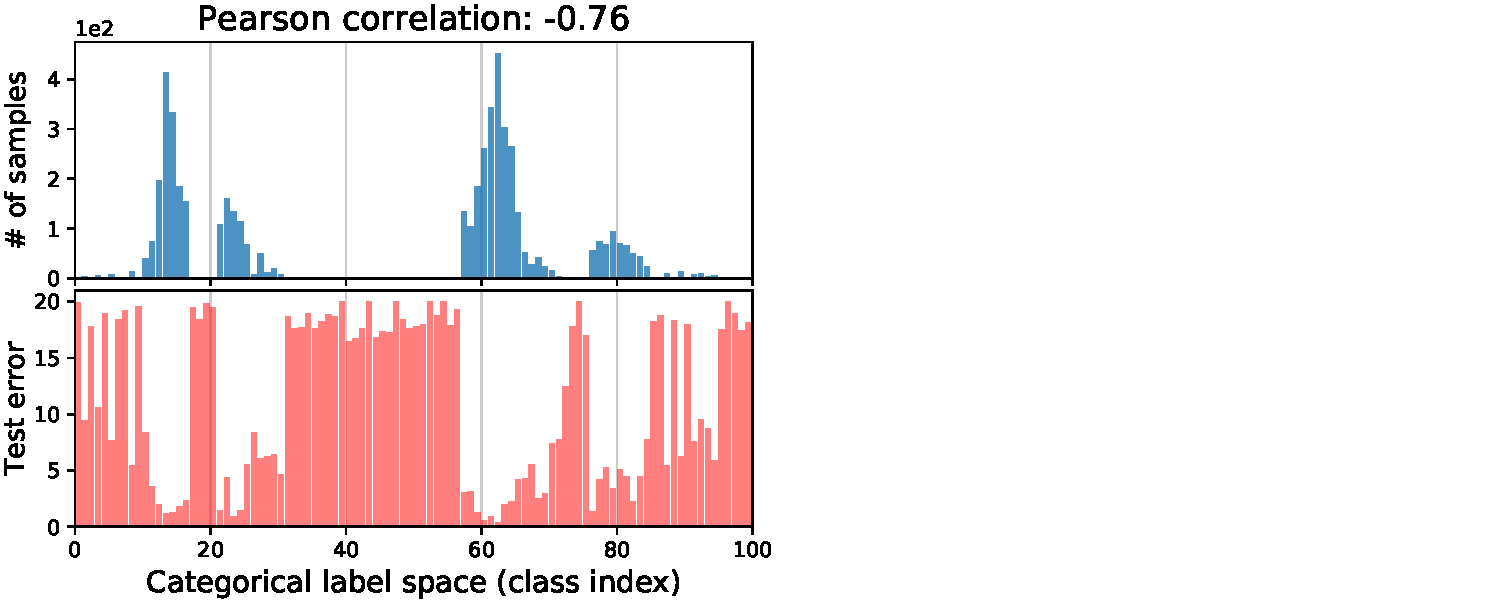
\includegraphics[width=\linewidth]{images/err_motivate_1_left.pdf}
			\caption{Classification}
		\end{subfigure}\hspace{1em}%
		\begin{subfigure}{0.44\textwidth}
			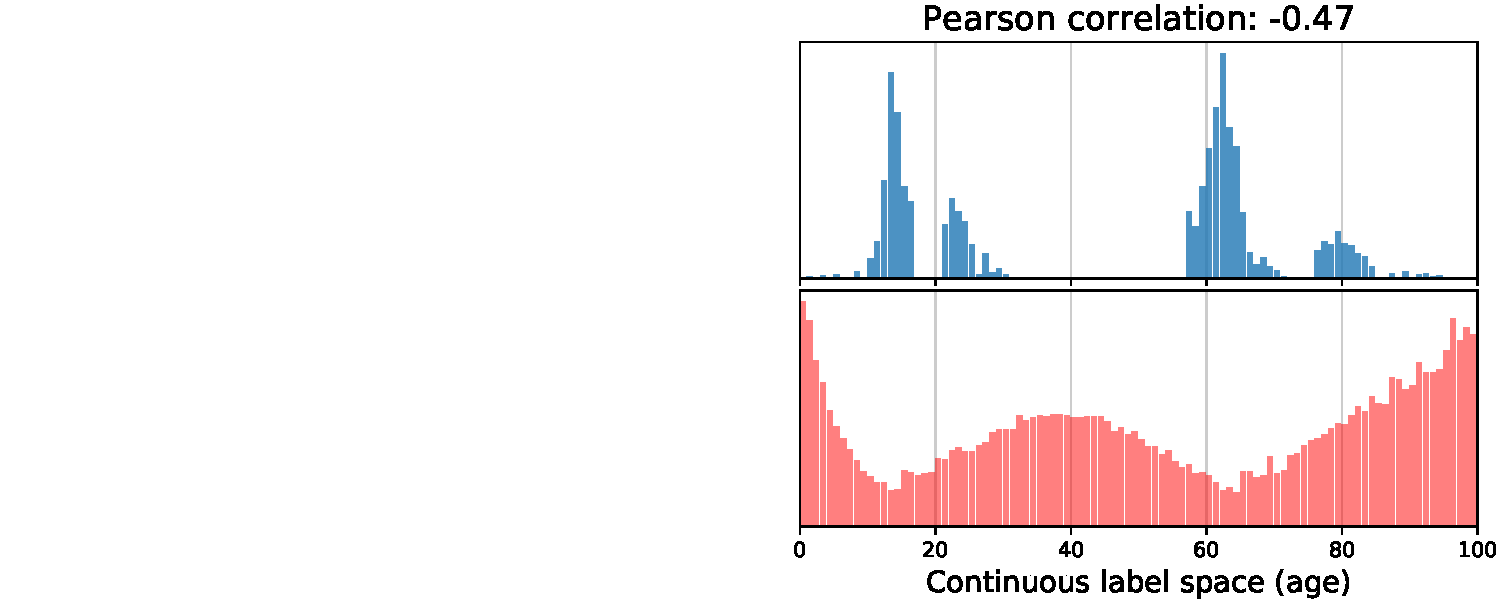
\includegraphics[width=\linewidth]{images/err_motivate_1_right.pdf}
			\caption{Regression}
		\end{subfigure}
		%\caption{}
	\end{figure}
	\footnotesize
	\vspace{-1.5em}
	\begin{columns}
		\begin{column}{0.5\textwidth}
			\begin{itemize}
				\item task: picture $\longrightarrow$ class
				\item data souce: CIFAR-100
			\end{itemize}
		\end{column}
		\begin{column}{0.5\textwidth}
			\begin{itemize}
				\item task: \\person's picture $\longrightarrow$ person's age
				\item age subrange: 0-99
				\item data souce: IMDB-WIKI
			\end{itemize}
		\end{column}
	\end{columns}
	\vspace{0.5em}
	\begin{itemize}
		\centering\item Simulated label imbalance
		\centering\item Label density distributions forced to be equal
		\centering\item Balanced test sets
	\end{itemize}
	\credit{Image}{yang2021delving}
\end{frame}

\begin{frame}{Imbalanced Categorical vs. Continuous Label Space (2/3)}
	\vspace{-2em}
	\begin{figure}[h]
		\begin{subfigure}{0.48\textwidth}
			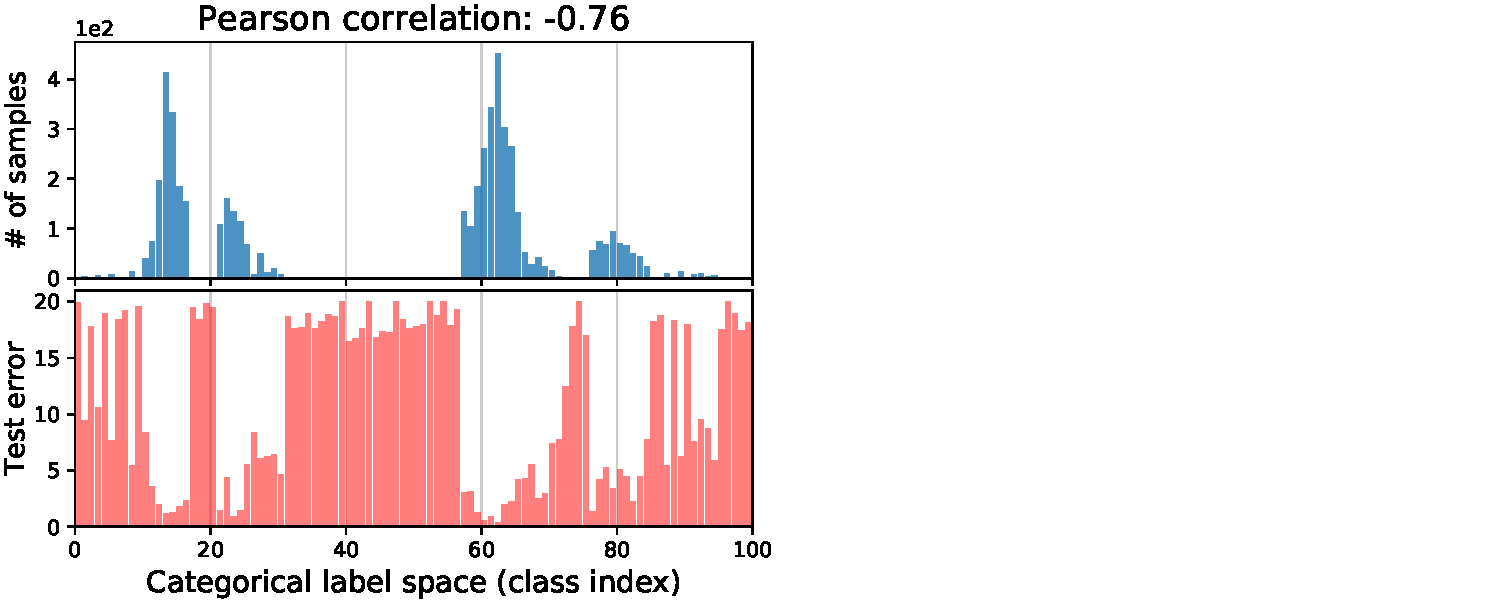
\includegraphics[width=\linewidth]{images/err_motivate_1_left.pdf}
			\caption{Classification}
		\end{subfigure}\hspace{1em}%
		\begin{subfigure}{0.44\textwidth}
			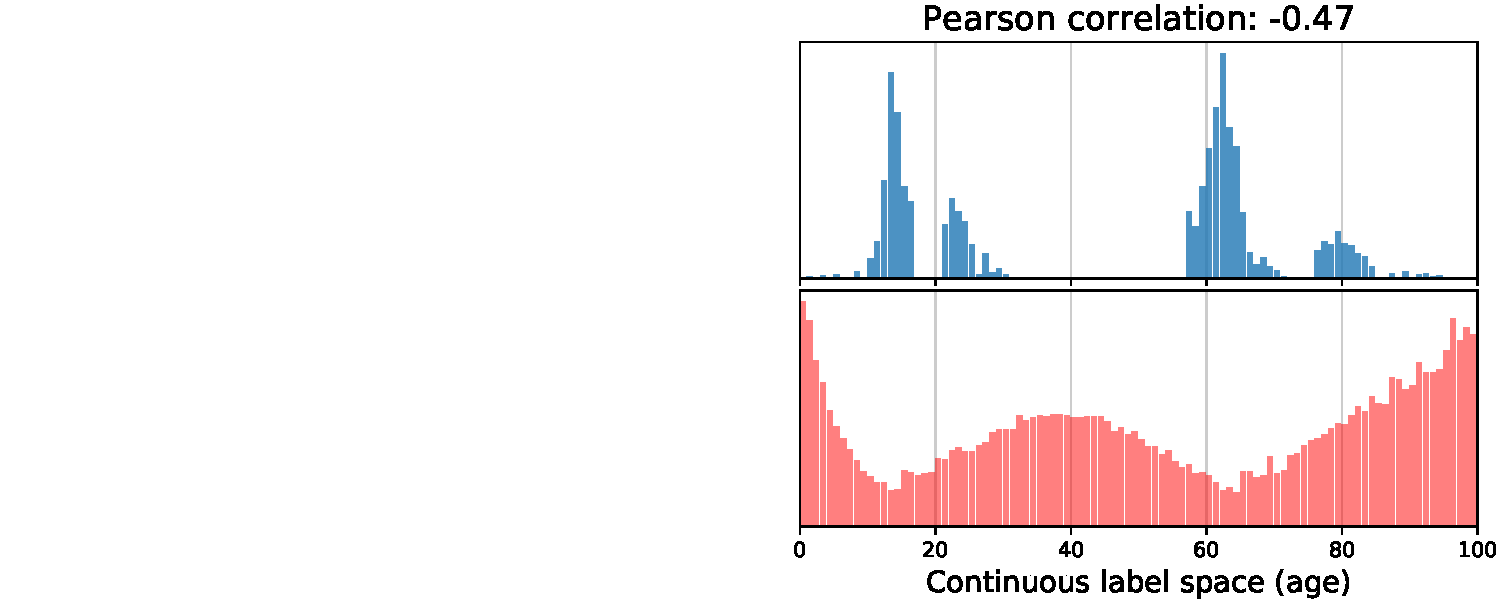
\includegraphics[width=\linewidth]{images/err_motivate_1_right.pdf}
			\caption{Regression}
		\end{subfigure}
		%\caption{}
	\end{figure}
	\footnotesize
	\vspace{-.5em}
	\begin{columns}
		\begin{column}{0.5\textwidth}
			\begin{itemize}
				\item the error distribution \emph{correlates} with the label density distribution
				\item majority classes with more examples are better learned than minority classes
			\end{itemize}
		\end{column}
		\begin{column}{0.5\textwidth}
			\begin{itemize}
				\item the error distribution DOES NOT \emph{correlate} well with the label density distribution
				\item smoother error distribution
			\end{itemize}
		\end{column}
	\end{columns}
	\credit{Image}{yang2021delving}
\end{frame}

\begin{frame}{Imbalanced Categorical vs. Continuous Label Space (3/3)}
	\vspace{-0.4em}
	\begin{figure}[h]
		\begin{subfigure}{0.48\textwidth}
			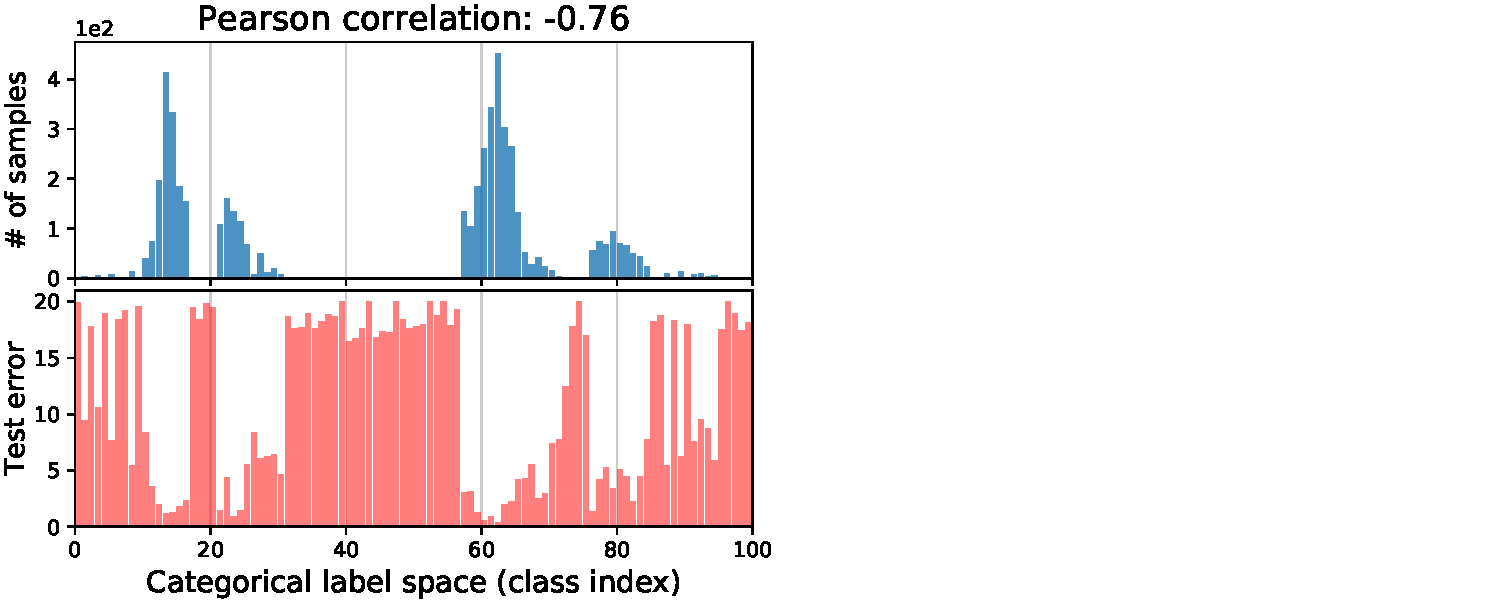
\includegraphics[width=\linewidth]{images/err_motivate_1_left.pdf}
			\caption{Classification}
		\end{subfigure}\hspace{1em}%
		\begin{subfigure}{0.44\textwidth}
			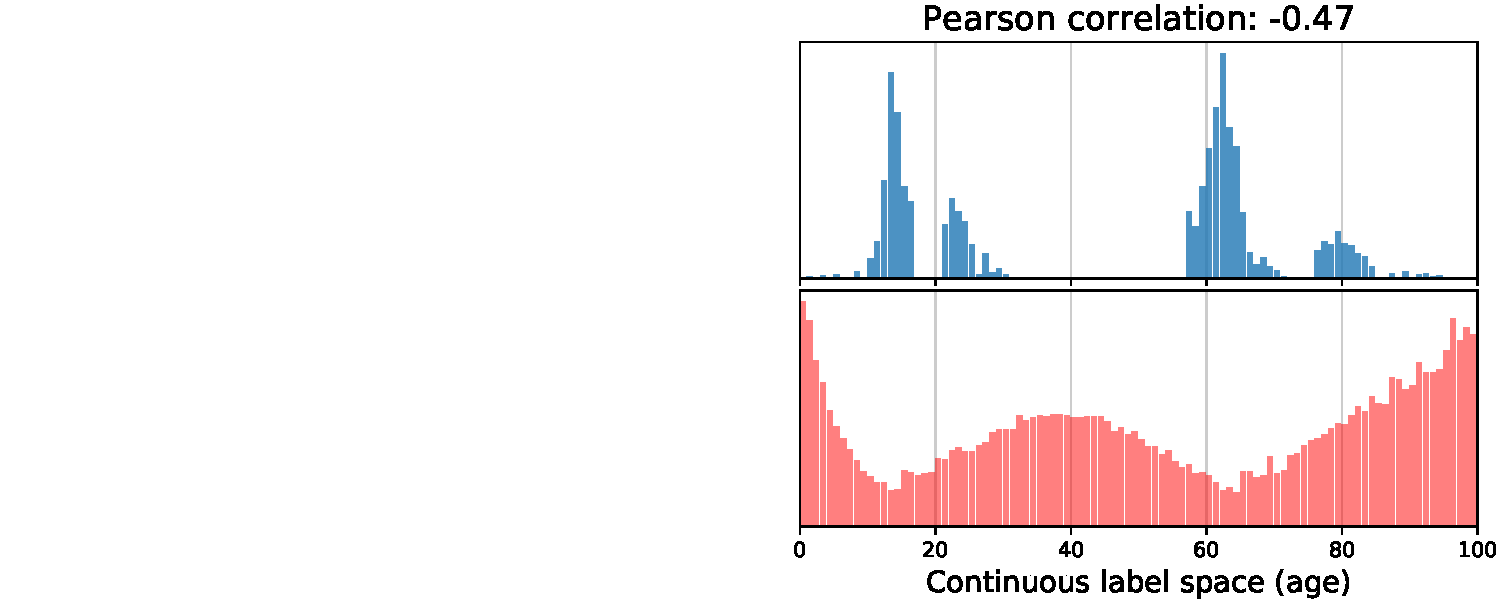
\includegraphics[width=\linewidth]{images/err_motivate_1_right.pdf}
			\caption{Regression}
		\end{subfigure}
		%\caption{}
	\end{figure}
	\vspace{-1em}
	\begin{columns}
		\fontsize{7pt}{7.2}\selectfont
		\begin{column}{0.5\textwidth}
			\begin{itemize}
				\item Compensating for the imbalance in the empirical label
				density distribution WORKS WELL.
			\end{itemize}
		\end{column}
		\begin{column}{0.5\textwidth}
			\begin{itemize}\setlength\itemsep{.5em}
				\item Compensating for the imbalance in the empirical label
				density distribution is INACCURATE.
				\item The empirical density does not accurately reflect the imbalance as seen by the model.
				\item Intuition: dependence between features at nearby labels.
				\item Proposed solution: \\\textbf{Label Distribution Smoothing (LDS)}
			\end{itemize}
		\end{column}
	\end{columns}
	\credit{Image}{yang2021delving}
\end{frame}

\begin{frame}{Label Distribution Smoothing (LDS) - Overview}
	\begin{figure}[h]
		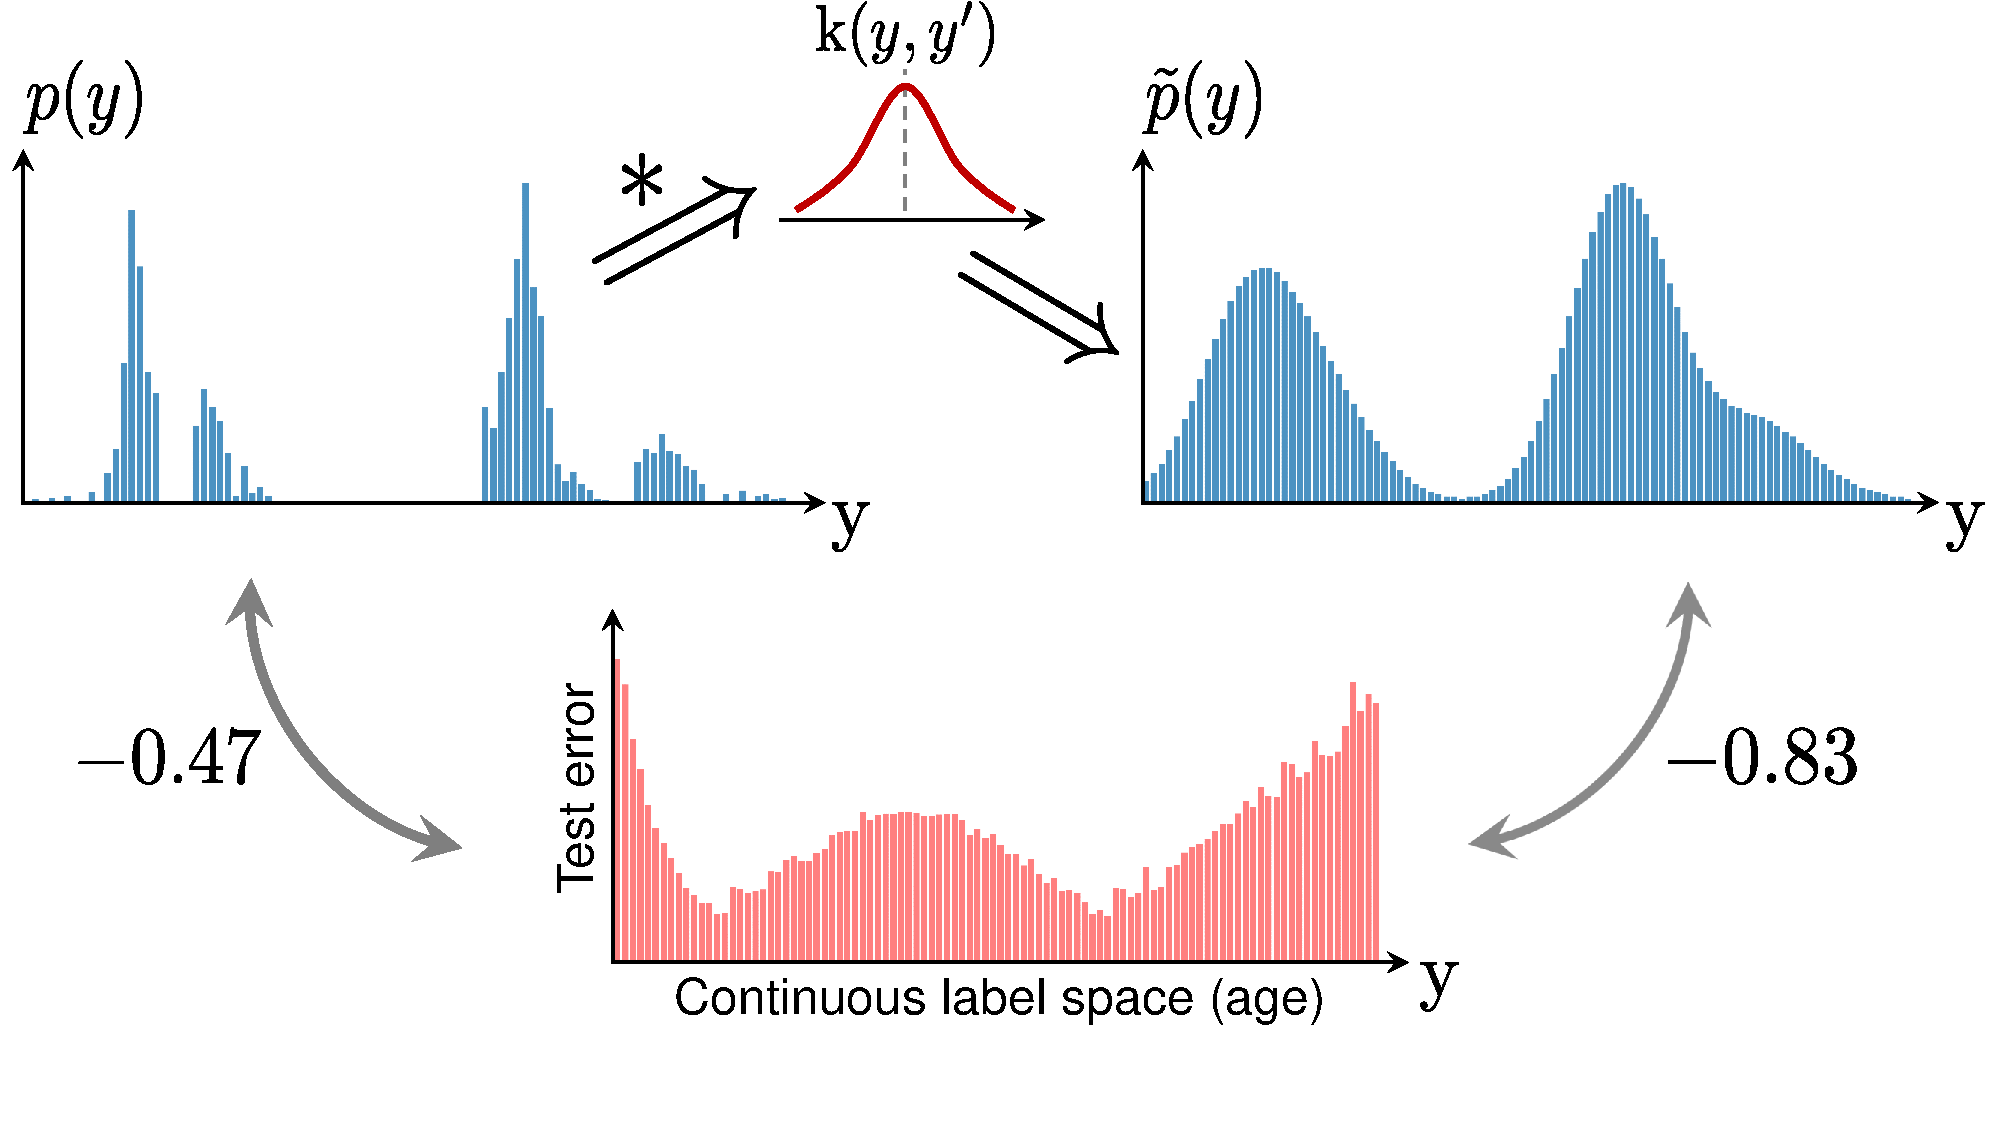
\includegraphics[width=\linewidth]{images/err_motivate_sep.pdf}
		%\caption{}
	\end{figure}
	\credit{Image}{yang2021delving}
\end{frame}

\begin{frame}[shrink=3]{Label Distribution Smoothing (LDS)}
	\begin{itemize}\setlength\itemsep{.5em}
		\item  Starting points
		\begin{itemize}
			\item Dependence between features at nearby continuous labels
			\item Expected density estimation
			\begin{itemize}
				\item Significant literature in statistics~(\cite{parzen1962estimation})
				\item Kernel density estimation
			\end{itemize}
		\end{itemize}
		\item Functioning
		\begin{itemize}
			\item Convolves a symmetric kernel with the empirical label density distribution.
			\item Extracts a kernel-smoothed label density accounting for the feature overlap of neighbouring labels.
		\end{itemize}
		\item Symmetric kernel
		\begin{itemize}
			\item E.g., Gaussian or Laplacian kernel
			\item Similarity between target values w.r.t. their distance in the target space.
		\end{itemize}
		\item \emph{Effective label density distribution}
		\begin{equation*}
			\tilde{p}(y') \triangleq \int_\mathcal{Y} k(y,y')p(y)dy
		\end{equation*}
		where 
		\begin{itemize}
			\item $p(y)$: nr. occurrences of label $y$ in training data
		\end{itemize}
		\item How to use it in practice?
		\begin{itemize}
			\item Possible direct adaptation of class imbalance techniques.
			\item E.g., loss weighted by inverse effective label density
		\end{itemize}
	\end{itemize}
\end{frame}